\chapter{Mô hình phân loại điện tâm đồ }
\thispagestyle{fancy}

\section{Giới thiệu về mô hình để xuất}

\begin{center}
    
\includegraphics[scale=.5]{image/chapter5/system.png}
    \begin{figure}[htp]
    \begin{center}
    \end{center}
    \caption{Sơ đồ hệ thống phân loại điện tâm đồ}
    \end{figure}
\end{center}

\section{Trích xuất đặc trưng tín hiệu điện tâm đồ}
Giai đoạn trích xuất đặc trưng được xem là chìa khóa thành công trong việc phát hiện bất thường. Việc trích xuất đặc trưng của điện tim là việc cực kỳ quan trọn, đặc trưng được trích xuất ra phải bao hàm một lượng thông tin đáng kể để mô hình phân loại có thể dựa vào những thông tin đó đưa ra những quyết định chính xác. Trong hệ thống này, khoảng R-R (R-R interval) được trích xuất và được xem là đặc trưng của ECG. Theo Clifford và các cộng sự \cite{rr_clifford}, khoảng R-R chứa rất nhiều thông tin quan trọng của tim, đặc biệt là những thông tin về tình trạng bất thường ở tim. Chính vì thế nhiều nghiên cứu trong việc phân loại tín hiệu điện tâm đồ , phát hiện bất thường ở tim mạch sử dụng thông tin khoảng R-R. Ling và Yang \cite{Lin2013} đã chỉ ra rằng việc sử dụng khoảng R-R chuẩn hóa cải thiện đáng kể kết quả việc phân loại tín hiệu điện tâm đồ.\par
Dữ liệu sau khi xử lý tiền dữ liệu sẽ được trích xuất đặc trưng bằng kỹ thuật ngưỡng thích ứng kết hợp được đề xuất bới Christov. Những điểm R trong dữ liệu sẽ được đánh nhãn R.
\begin{center}
    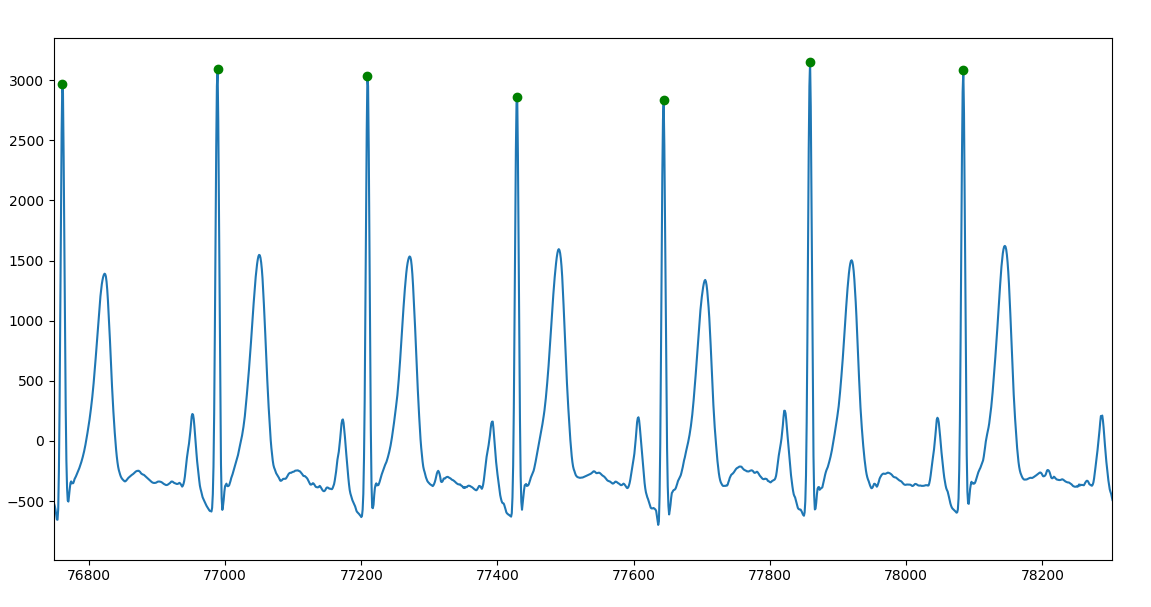
\includegraphics[scale=.3]{image/chapter5/R_detect.png}
    \begin{figure}[htp]
    \begin{center}
    \end{center}
    \caption{Hình ảnh đỉnh R được đánh dấu}
    \end{figure}
\end{center}

\section{Xử lý tín hiệu (khử nhiễu)}
Tín hiệu điện tâm đồ khi được thu nhận từ các thiết bị đo ban đầu có khả năng rất cao bị nhiễu do nhiều yếu tố khác nhau, như nhiễu do ảnh hưởng từ cơ bắp, nhiễu sinh ra từ các thiết bị điện tử, nhiễu từ các điện cực của thiết bị đo điện tâm đồ, power line interference, baseline wander,… Nhiễu có tác động rất lớn đến chất lượng của việc trích xuất đặc trưng và do đó ảnh hưởng đến kết quả bài toán phân loại (việc trích xuất đặc trưng từ tín hiệu điện tâm đồ có thể không chính xác và do đó có thể dẫn đến kết quả phân loại, chẩn đoán bị sai). Vì vậy, tín hiệu điện tâm đồ được thu nhận lúc ban đầu cần phải được khử nhiễu trước khi được thực hiện các bước trích xuất đặc trưng và phân loại. Giải pháp cho việc khử nhiễu đó là lọc nhiễu Butterworth bậc 2 gồm high pass, low pass.
\begin{center}
         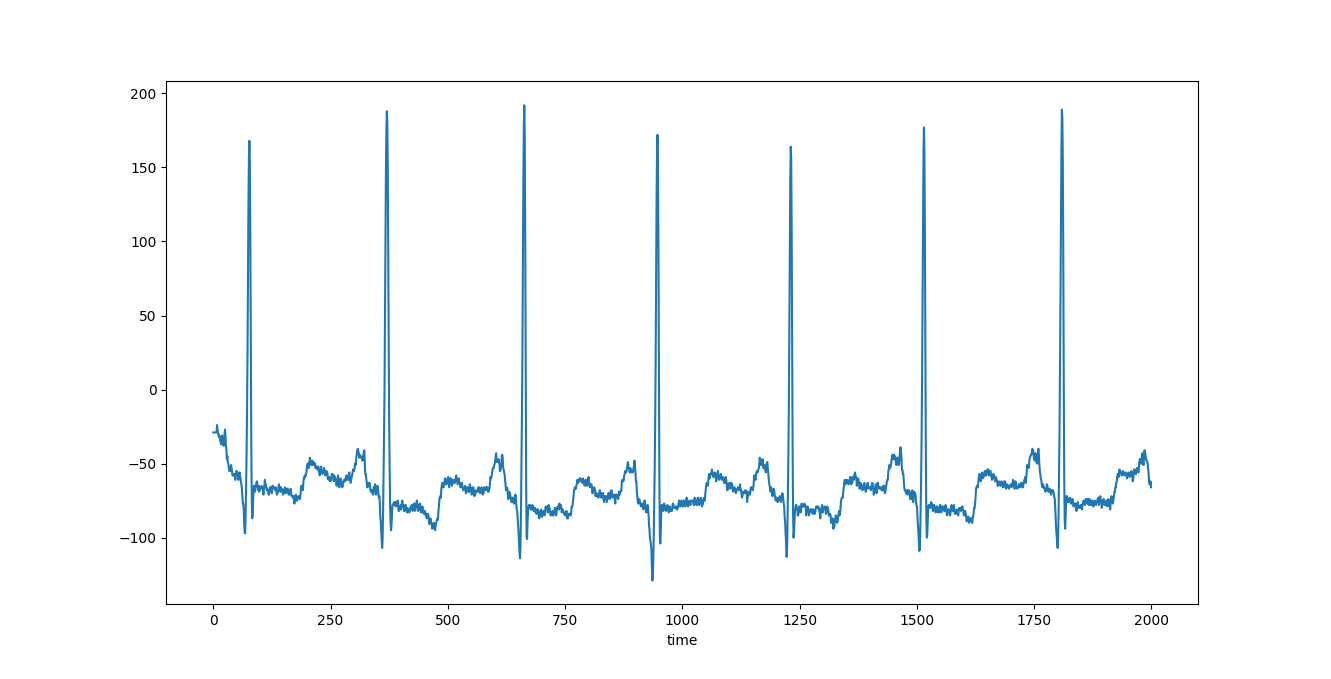
\includegraphics[width=.9\linewidth]{image/chapter5/noise.png}
         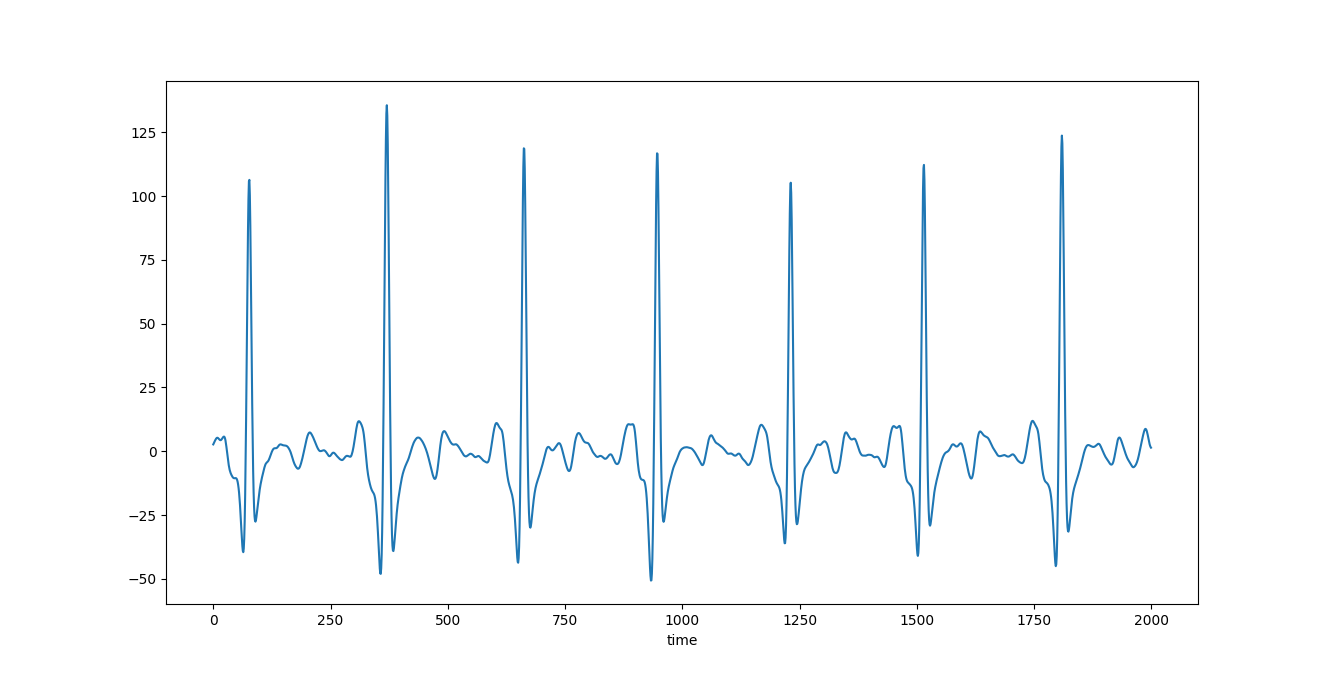
\includegraphics[width=.9\linewidth]{image/chapter5/hlp.png}
    \begin{figure}[!htb]
       \caption{Dữ liệu trước và sau khi lọc nhiễu}
    \end{figure}
\end{center}

\section{Chuẩn hóa đặc trưng độ dài và biên độ khoảng R-R }
Một trong những bước đặc biệt và có ảnh hưởng rất lớn đến chất lượng phân loại tín hiệu điện tâm đồ trong nghiên cứu này là việc chuẩn hóa hình dạng (shape normalization) cho đặc trưng khoảng R-R. Do đặc điểm sinh lý của tim mà các khoảng R-R thường có độ dài khác nhau (nhịp đập của tim thường không bất biến mà sẽ có một sự chênh lệch nhất định). Ở người bình thường, không mắc các bệnh lý về tim mạch, khoảng R-R sẽ dao động trong khoảng 600 – 1200 ms \cite{64} . Nếu sự không đồng nhất về mặt hình dạng của các khoảng R-R này không được giải quyết hiệu quả thì việc phân loại những tín hiệu điện tâm đồ mới, không có trong tập dữ liệu huấn luyện, sẽ gặp khó khăn và có thể dẫn đến kết quả phân loại, chẩn đoán không còn chính xác (trường hợp này được gọi là overfit – mô hình phân loại chỉ đáp ứng tốt với dữ liệu huấn luyện mà không còn đáp ứng tốt với dữ liệu kiểm thử hoàn toàn mới). Đó là lý do vì sao các khoảng R-R cần phải được chuẩn hóa về một hình dạng nhất định. Massagram và nhóm nghiên cứu \cite{67}, Bhola và nhóm nghiên cứu đều cho rằng 880 – 900 ms là khoảng thời gian phổ biến nhất của khoảng R-R \cite{68}.\par
Do đó, toàn bộ khoảng R-R trong nghiên cứu này sẽ được chuẩn hóa về khoảng thời gian đồng nhất 900 ms bằng phương pháp nội suy tuyến tính (linear interpolation). Hình dạng của khoảng R-R sau khi đã được chuẩn hóa đồng nhất về cùng một khoảng nhất định sẽ gần như không sai lệch quá nhiều so với khoảng R-R ban đầu. Điều này đồng nghĩa với việc mỗi đoạn R-R sẽ có 324 samples dữ liệu.\par


\section{Phân loại tín hiệu điện tâm đồ}
Mô hìn phân loại tín hiệu điện tâm đồ gồm sự kết hợp giữa mạng LSTM và tầng Fully-connected. Trong đó:
\begin{itemize}
    \item Mạng LSTM ở phần đầu của mô hình có chức năng học những đặc trưng tín hiệu điện tâm đồ có dạng Sequence-to-Sequence (Seq2Seq). 
    \item Tầng Fully-connected có chức năng phân loại phân loại đã được học thành 2 nhãn Bình thường (0) và Bất thường (1).
\end{itemize}
\begin{center}
    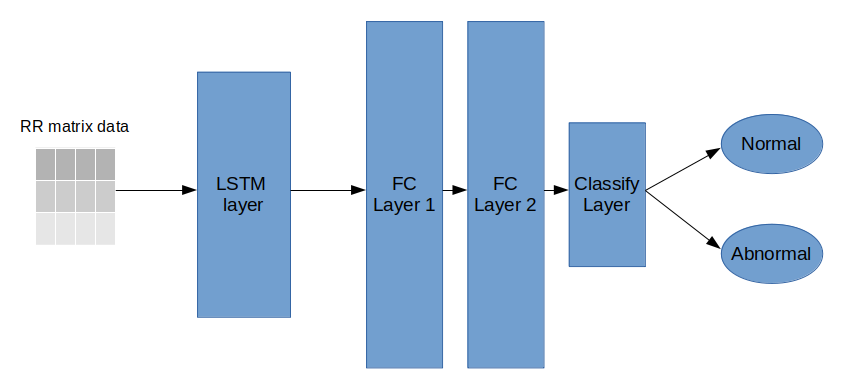
\includegraphics[scale=.4]{image/chapter5/model_architechture.png}
    \begin{figure}[htp]
    \begin{center}
    \end{center}
    \caption{Kiến trúc mô hình phân loại}
    \end{figure}
\end{center}
Các tham số của mô hình phân loại:

\textbf{Tham số tốc độ học (learning rate)}: là 0.001 trên nguyên tắc thử sai nhiều lần, giá trị này ảnh hưởng đến tốc độ hội tụ của quá trình huấn luyện. (tốc độ học là một siêu tham số  được sử dụng trong đào tạo mạng lưới thần kinh có giá trị dương nhỏ, thường nằm trong khoảng giữa 0,0 và 1,0)\par
\textbf{Tầng Fully-Connected}: bao gồm 2 layer với 20 neural ẩn mỗi layer.\par
\textbf{Hàm biến đổi softmax} được áp dụng để phân loại 2 nhãn được gán đối với mỗi dữ liệu.\par
$S(y_i) = \frac{e^{y_i}}{\sum_{j=1}^{j}e^{y_i}}$ \par

\textbf{Hàm lỗi Cross-entropy} được sử dụng để phân loại nhãn Bình thường và Bất thường.\par
$L(y,p)=-\sum_{C}^{i=1}y_i\ln(p_i)$\par
\textbf{Các kỹ thuật tránh overfit} được áp dụng trên 2 layer Fully-connected để tránh overfitting dẫn đến sự sai lệch trong việc kiểm thử dữ liệu.
\begin{itemize}
    \item Chính quy hóa L2 (Relularization L2)
    \item Dropout
    \item Early Stopping
    \item Khởi tạo trọng số kiểu Xavier.
\end{itemize}\par
\textbf{Phương pháp tối ưu hóa hàm lỗi}: bộ tối ưu Adam.\par
\textbf{Số lần tính toán (epoch): 100}
